% Title: Block diagram of Third order noise shaper in Compact Disc Players
% Author: Ramón Jaramillo
\documentclass{article}

\usepackage{tikz}
%\usepackage{textcomp}
\begin{document}



\begin{figure}[t]
\centering
% Created by tikzDevice version 0.11 on 2018-04-15 12:26:52
% !TEX encoding = UTF-8 Unicode
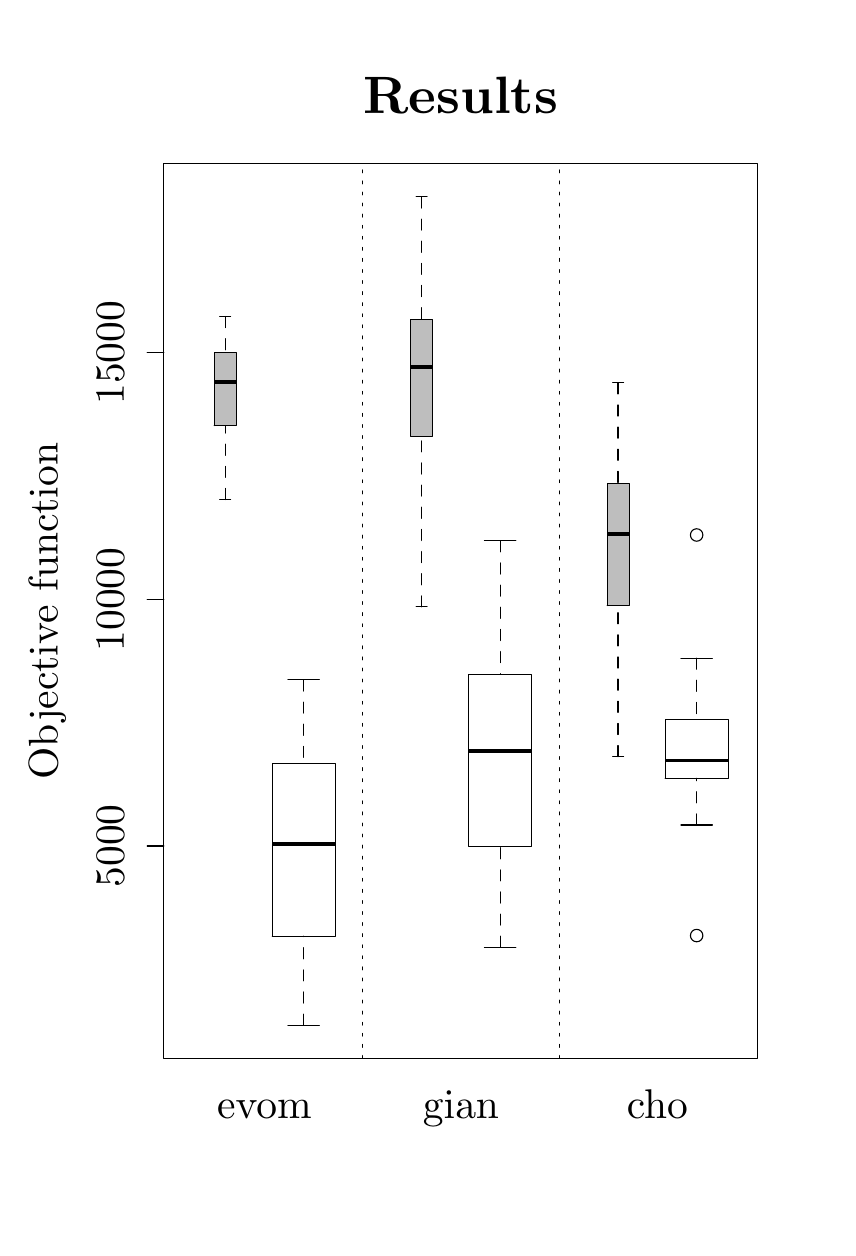
\begin{tikzpicture}[x=1pt,y=1pt]
\definecolor{fillColor}{RGB}{255,255,255}
\path[use as bounding box,fill=fillColor,fill opacity=0.00] (0,0) rectangle (289.08,433.62);
\begin{scope}
\path[clip] ( 49.20, 61.20) rectangle (263.88,384.42);
\definecolor{fillColor}{RGB}{190,190,190}

\path[fill=fillColor] ( 67.37,289.82) --
	( 75.33,289.82) --
	( 75.33,316.10) --
	( 67.37,316.10) --
	cycle;
\definecolor{drawColor}{RGB}{0,0,0}

\path[draw=drawColor,line width= 1.2pt,line join=round] ( 67.37,305.56) -- ( 75.33,305.56);

\path[draw=drawColor,line width= 0.4pt,dash pattern=on 4pt off 4pt ,line join=round,line cap=round] ( 71.35,263.11) -- ( 71.35,289.82);

\path[draw=drawColor,line width= 0.4pt,dash pattern=on 4pt off 4pt ,line join=round,line cap=round] ( 71.35,329.23) -- ( 71.35,316.10);

\path[draw=drawColor,line width= 0.4pt,line join=round,line cap=round] ( 69.36,263.11) -- ( 73.34,263.11);

\path[draw=drawColor,line width= 0.4pt,line join=round,line cap=round] ( 69.36,329.23) -- ( 73.34,329.23);

\path[draw=drawColor,line width= 0.4pt,line join=round,line cap=round] ( 67.37,289.82) --
	( 75.33,289.82) --
	( 75.33,316.10) --
	( 67.37,316.10) --
	( 67.37,289.82);
\definecolor{fillColor}{RGB}{255,255,255}

\path[fill=fillColor] ( 88.39,105.37) --
	(111.11,105.37) --
	(111.11,167.75) --
	( 88.39,167.75) --
	cycle;

\path[draw=drawColor,line width= 1.2pt,line join=round] ( 88.39,138.63) -- (111.11,138.63);

\path[draw=drawColor,line width= 0.4pt,dash pattern=on 4pt off 4pt ,line join=round,line cap=round] ( 99.75, 73.17) -- ( 99.75,105.37);

\path[draw=drawColor,line width= 0.4pt,dash pattern=on 4pt off 4pt ,line join=round,line cap=round] ( 99.75,197.92) -- ( 99.75,167.75);

\path[draw=drawColor,line width= 0.4pt,line join=round,line cap=round] ( 94.07, 73.17) -- (105.43, 73.17);

\path[draw=drawColor,line width= 0.4pt,line join=round,line cap=round] ( 94.07,197.92) -- (105.43,197.92);

\path[draw=drawColor,line width= 0.4pt,line join=round,line cap=round] ( 88.39,105.37) --
	(111.11,105.37) --
	(111.11,167.75) --
	( 88.39,167.75) --
	( 88.39,105.37);
\definecolor{fillColor}{RGB}{190,190,190}

\path[fill=fillColor] (138.37,286.01) --
	(146.32,286.01) --
	(146.32,328.30) --
	(138.37,328.30) --
	cycle;

\path[draw=drawColor,line width= 1.2pt,line join=round] (138.37,311.00) -- (146.32,311.00);

\path[draw=drawColor,line width= 0.4pt,dash pattern=on 4pt off 4pt ,line join=round,line cap=round] (142.34,224.32) -- (142.34,286.01);

\path[draw=drawColor,line width= 0.4pt,dash pattern=on 4pt off 4pt ,line join=round,line cap=round] (142.34,372.45) -- (142.34,328.30);

\path[draw=drawColor,line width= 0.4pt,line join=round,line cap=round] (140.35,224.32) -- (144.33,224.32);

\path[draw=drawColor,line width= 0.4pt,line join=round,line cap=round] (140.35,372.45) -- (144.33,372.45);

\path[draw=drawColor,line width= 0.4pt,line join=round,line cap=round] (138.37,286.01) --
	(146.32,286.01) --
	(146.32,328.30) --
	(138.37,328.30) --
	(138.37,286.01);
\definecolor{fillColor}{RGB}{255,255,255}

\path[fill=fillColor] (159.38,137.89) --
	(182.10,137.89) --
	(182.10,199.95) --
	(159.38,199.95) --
	cycle;

\path[draw=drawColor,line width= 1.2pt,line join=round] (159.38,172.19) -- (182.10,172.19);

\path[draw=drawColor,line width= 0.4pt,dash pattern=on 4pt off 4pt ,line join=round,line cap=round] (170.74,101.31) -- (170.74,137.89);

\path[draw=drawColor,line width= 0.4pt,dash pattern=on 4pt off 4pt ,line join=round,line cap=round] (170.74,248.18) -- (170.74,199.95);

\path[draw=drawColor,line width= 0.4pt,line join=round,line cap=round] (165.06,101.31) -- (176.42,101.31);

\path[draw=drawColor,line width= 0.4pt,line join=round,line cap=round] (165.06,248.18) -- (176.42,248.18);

\path[draw=drawColor,line width= 0.4pt,line join=round,line cap=round] (159.38,137.89) --
	(182.10,137.89) --
	(182.10,199.95) --
	(159.38,199.95) --
	(159.38,137.89);
\definecolor{fillColor}{RGB}{190,190,190}

\path[fill=fillColor] (209.36,224.79) --
	(217.31,224.79) --
	(217.31,268.80) --
	(209.36,268.80) --
	cycle;

\path[draw=drawColor,line width= 1.2pt,line join=round] (209.36,250.64) -- (217.31,250.64);

\path[draw=drawColor,line width= 0.4pt,dash pattern=on 4pt off 4pt ,line join=round,line cap=round] (213.33,170.21) -- (213.33,224.79);

\path[draw=drawColor,line width= 0.4pt,dash pattern=on 4pt off 4pt ,line join=round,line cap=round] (213.33,305.28) -- (213.33,268.80);

\path[draw=drawColor,line width= 0.4pt,line join=round,line cap=round] (211.35,170.21) -- (215.32,170.21);

\path[draw=drawColor,line width= 0.4pt,line join=round,line cap=round] (211.35,305.28) -- (215.32,305.28);

\path[draw=drawColor,line width= 0.4pt,line join=round,line cap=round] (209.36,224.79) --
	(217.31,224.79) --
	(217.31,268.80) --
	(209.36,268.80) --
	(209.36,224.79);
\definecolor{fillColor}{RGB}{255,255,255}

\path[fill=fillColor] (230.37,162.38) --
	(253.09,162.38) --
	(253.09,183.52) --
	(230.37,183.52) --
	cycle;

\path[draw=drawColor,line width= 1.2pt,line join=round] (230.37,168.93) -- (253.09,168.93);

\path[draw=drawColor,line width= 0.4pt,dash pattern=on 4pt off 4pt ,line join=round,line cap=round] (241.73,145.51) -- (241.73,162.38);

\path[draw=drawColor,line width= 0.4pt,dash pattern=on 4pt off 4pt ,line join=round,line cap=round] (241.73,205.80) -- (241.73,183.52);

\path[draw=drawColor,line width= 0.4pt,line join=round,line cap=round] (236.05,145.51) -- (247.41,145.51);

\path[draw=drawColor,line width= 0.4pt,line join=round,line cap=round] (236.05,205.80) -- (247.41,205.80);

\path[draw=drawColor,line width= 0.4pt,line join=round,line cap=round] (230.37,162.38) --
	(253.09,162.38) --
	(253.09,183.52) --
	(230.37,183.52) --
	(230.37,162.38);

\path[draw=drawColor,line width= 0.4pt,line join=round,line cap=round] (241.73,105.55) circle (  2.25);

\path[draw=drawColor,line width= 0.4pt,line join=round,line cap=round] (241.73,250.30) circle (  2.25);
\end{scope}
\begin{scope}
\path[clip] (  0.00,  0.00) rectangle (289.08,433.62);
\definecolor{drawColor}{RGB}{0,0,0}

\node[text=drawColor,rotate= 90.00,anchor=base,inner sep=0pt, outer sep=0pt, scale=  1.50] at ( 10.80,222.81) {Objective function};
\end{scope}
\begin{scope}
\path[clip] ( 49.20, 61.20) rectangle (263.88,384.42);
\definecolor{drawColor}{RGB}{0,0,0}

\path[draw=drawColor,line width= 0.4pt,dash pattern=on 1pt off 3pt ,line join=round,line cap=round] (121.04, 61.20) -- (121.04,384.42);

\path[draw=drawColor,line width= 0.4pt,dash pattern=on 1pt off 3pt ,line join=round,line cap=round] (192.04, 61.20) -- (192.04,384.42);
\end{scope}
\begin{scope}
\path[clip] (  0.00,  0.00) rectangle (289.08,433.62);
\definecolor{drawColor}{RGB}{0,0,0}

\node[text=drawColor,anchor=base,inner sep=0pt, outer sep=0pt, scale=  1.50] at ( 85.55, 39.60) {evom};

\node[text=drawColor,anchor=base,inner sep=0pt, outer sep=0pt, scale=  1.50] at (156.54, 39.60) {gian};

\node[text=drawColor,anchor=base,inner sep=0pt, outer sep=0pt, scale=  1.50] at (227.53, 39.60) {cho};
\end{scope}
\begin{scope}
\path[clip] (  0.00,  0.00) rectangle (289.08,433.62);
\definecolor{drawColor}{RGB}{0,0,0}

\node[text=drawColor,anchor=base,inner sep=0pt, outer sep=0pt, scale=  1.90] at (156.54,402.46) {\bfseries Results};
\end{scope}
\begin{scope}
\path[clip] (  0.00,  0.00) rectangle (289.08,433.62);
\definecolor{drawColor}{RGB}{0,0,0}

\path[draw=drawColor,line width= 0.4pt,line join=round,line cap=round] ( 49.20,137.92) -- ( 49.20,316.13);

\path[draw=drawColor,line width= 0.4pt,line join=round,line cap=round] ( 49.20,137.92) -- ( 43.20,137.92);

\path[draw=drawColor,line width= 0.4pt,line join=round,line cap=round] ( 49.20,227.02) -- ( 43.20,227.02);

\path[draw=drawColor,line width= 0.4pt,line join=round,line cap=round] ( 49.20,316.13) -- ( 43.20,316.13);

\node[text=drawColor,rotate= 90.00,anchor=base,inner sep=0pt, outer sep=0pt, scale=  1.50] at ( 34.80,137.92) {5000};

\node[text=drawColor,rotate= 90.00,anchor=base,inner sep=0pt, outer sep=0pt, scale=  1.50] at ( 34.80,227.02) {10000};

\node[text=drawColor,rotate= 90.00,anchor=base,inner sep=0pt, outer sep=0pt, scale=  1.50] at ( 34.80,316.13) {15000};

\path[draw=drawColor,line width= 0.4pt,line join=round,line cap=round] ( 49.20, 61.20) --
	(263.88, 61.20) --
	(263.88,384.42) --
	( 49.20,384.42) --
	( 49.20, 61.20);
\end{scope}
\end{tikzpicture}

\hfill
% Created by tikzDevice version 0.11 on 2018-04-09 15:27:55
% !TEX encoding = UTF-8 Unicode
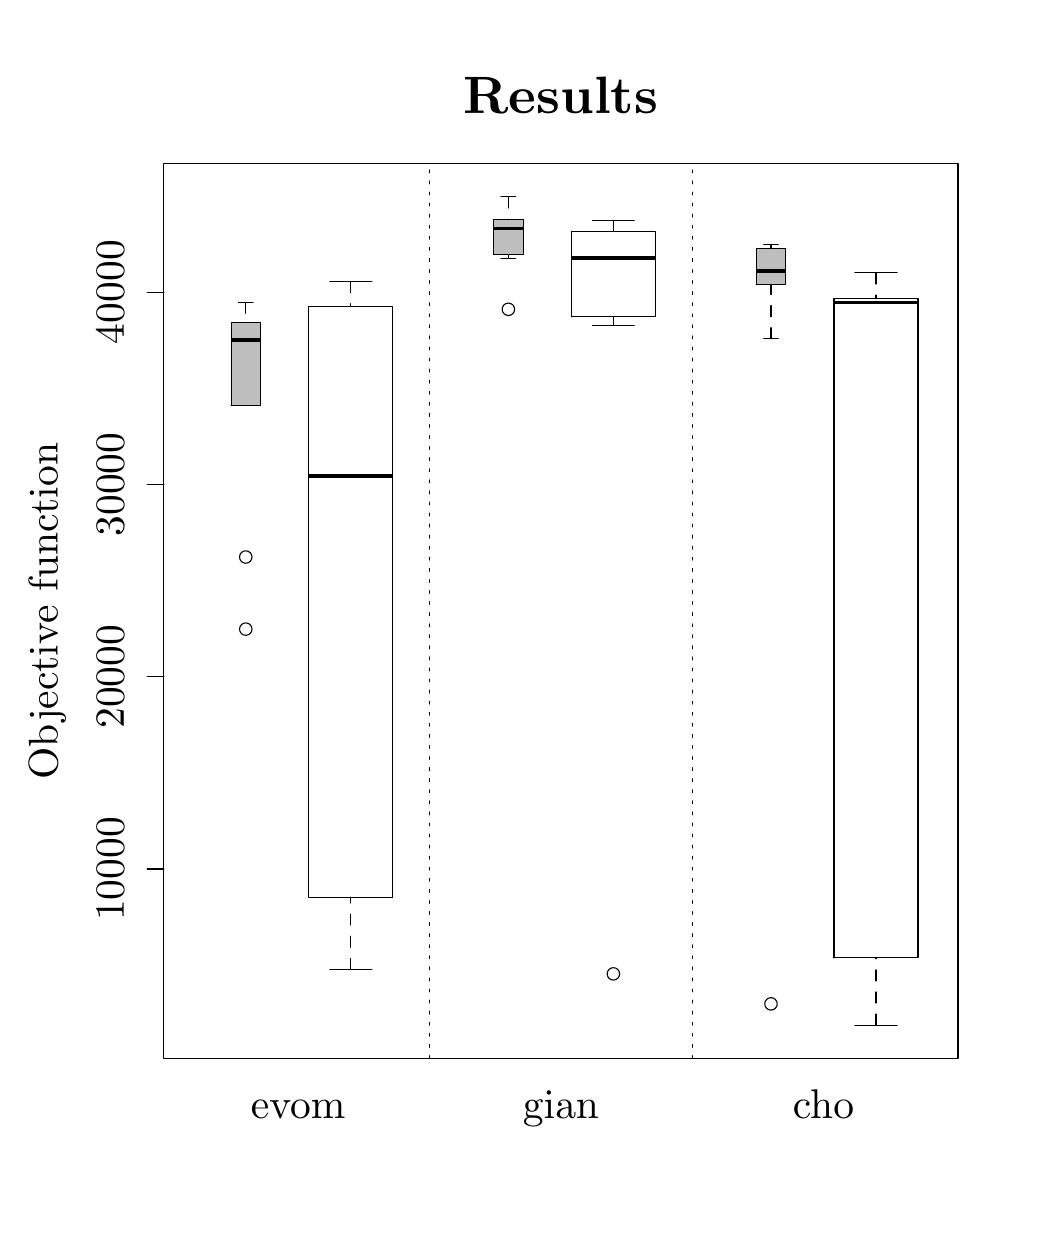
\begin{tikzpicture}[x=1pt,y=1pt]
\definecolor{fillColor}{RGB}{255,255,255}
\path[use as bounding box,fill=fillColor,fill opacity=0.00] (0,0) rectangle (361.35,433.62);
\begin{scope}
\path[clip] ( 49.20, 61.20) rectangle (336.15,384.42);
\definecolor{fillColor}{RGB}{190,190,190}

\path[fill=fillColor] ( 73.49,297.05) --
	( 84.12,297.05) --
	( 84.12,327.09) --
	( 73.49,327.09) --
	cycle;
\definecolor{drawColor}{RGB}{0,0,0}

\path[draw=drawColor,line width= 1.2pt,line join=round] ( 73.49,320.70) -- ( 84.12,320.70);

\path[draw=drawColor,line width= 0.4pt,dash pattern=on 4pt off 4pt ,line join=round,line cap=round] ( 78.81,297.05) -- ( 78.81,297.05);

\path[draw=drawColor,line width= 0.4pt,dash pattern=on 4pt off 4pt ,line join=round,line cap=round] ( 78.81,334.37) -- ( 78.81,327.09);

\path[draw=drawColor,line width= 0.4pt,line join=round,line cap=round] ( 76.15,297.05) -- ( 81.46,297.05);

\path[draw=drawColor,line width= 0.4pt,line join=round,line cap=round] ( 76.15,334.37) -- ( 81.46,334.37);

\path[draw=drawColor,line width= 0.4pt,line join=round,line cap=round] ( 73.49,297.05) --
	( 84.12,297.05) --
	( 84.12,327.09) --
	( 73.49,327.09) --
	( 73.49,297.05);

\path[draw=drawColor,line width= 0.4pt,line join=round,line cap=round] ( 78.81,242.33) circle (  2.25);

\path[draw=drawColor,line width= 0.4pt,line join=round,line cap=round] ( 78.81,216.29) circle (  2.25);
\definecolor{fillColor}{RGB}{255,255,255}

\path[fill=fillColor] (101.58,119.42) --
	(131.94,119.42) --
	(131.94,332.86) --
	(101.58,332.86) --
	cycle;

\path[draw=drawColor,line width= 1.2pt,line join=round] (101.58,271.60) -- (131.94,271.60);

\path[draw=drawColor,line width= 0.4pt,dash pattern=on 4pt off 4pt ,line join=round,line cap=round] (116.76, 93.32) -- (116.76,119.42);

\path[draw=drawColor,line width= 0.4pt,dash pattern=on 4pt off 4pt ,line join=round,line cap=round] (116.76,341.86) -- (116.76,332.86);

\path[draw=drawColor,line width= 0.4pt,line join=round,line cap=round] (109.17, 93.32) -- (124.35, 93.32);

\path[draw=drawColor,line width= 0.4pt,line join=round,line cap=round] (109.17,341.86) -- (124.35,341.86);

\path[draw=drawColor,line width= 0.4pt,line join=round,line cap=round] (101.58,119.42) --
	(131.94,119.42) --
	(131.94,332.86) --
	(101.58,332.86) --
	(101.58,119.42);
\definecolor{fillColor}{RGB}{190,190,190}

\path[fill=fillColor] (168.38,351.63) --
	(179.01,351.63) --
	(179.01,364.37) --
	(168.38,364.37) --
	cycle;

\path[draw=drawColor,line width= 1.2pt,line join=round] (168.38,361.13) -- (179.01,361.13);

\path[draw=drawColor,line width= 0.4pt,dash pattern=on 4pt off 4pt ,line join=round,line cap=round] (173.70,350.16) -- (173.70,351.63);

\path[draw=drawColor,line width= 0.4pt,dash pattern=on 4pt off 4pt ,line join=round,line cap=round] (173.70,372.45) -- (173.70,364.37);

\path[draw=drawColor,line width= 0.4pt,line join=round,line cap=round] (171.04,350.16) -- (176.35,350.16);

\path[draw=drawColor,line width= 0.4pt,line join=round,line cap=round] (171.04,372.45) -- (176.35,372.45);

\path[draw=drawColor,line width= 0.4pt,line join=round,line cap=round] (168.38,351.63) --
	(179.01,351.63) --
	(179.01,364.37) --
	(168.38,364.37) --
	(168.38,351.63);

\path[draw=drawColor,line width= 0.4pt,line join=round,line cap=round] (173.70,331.85) circle (  2.25);
\definecolor{fillColor}{RGB}{255,255,255}

\path[fill=fillColor] (196.47,329.15) --
	(226.84,329.15) --
	(226.84,359.82) --
	(196.47,359.82) --
	cycle;

\path[draw=drawColor,line width= 1.2pt,line join=round] (196.47,350.33) -- (226.84,350.33);

\path[draw=drawColor,line width= 0.4pt,dash pattern=on 4pt off 4pt ,line join=round,line cap=round] (211.65,326.04) -- (211.65,329.15);

\path[draw=drawColor,line width= 0.4pt,dash pattern=on 4pt off 4pt ,line join=round,line cap=round] (211.65,363.98) -- (211.65,359.82);

\path[draw=drawColor,line width= 0.4pt,line join=round,line cap=round] (204.06,326.04) -- (219.24,326.04);

\path[draw=drawColor,line width= 0.4pt,line join=round,line cap=round] (204.06,363.98) -- (219.24,363.98);

\path[draw=drawColor,line width= 0.4pt,line join=round,line cap=round] (196.47,329.15) --
	(226.84,329.15) --
	(226.84,359.82) --
	(196.47,359.82) --
	(196.47,329.15);

\path[draw=drawColor,line width= 0.4pt,line join=round,line cap=round] (211.65, 91.71) circle (  2.25);
\definecolor{fillColor}{RGB}{190,190,190}

\path[fill=fillColor] (263.27,340.73) --
	(273.90,340.73) --
	(273.90,353.79) --
	(263.27,353.79) --
	cycle;

\path[draw=drawColor,line width= 1.2pt,line join=round] (263.27,345.66) -- (273.90,345.66);

\path[draw=drawColor,line width= 0.4pt,dash pattern=on 4pt off 4pt ,line join=round,line cap=round] (268.59,321.20) -- (268.59,340.73);

\path[draw=drawColor,line width= 0.4pt,dash pattern=on 4pt off 4pt ,line join=round,line cap=round] (268.59,355.32) -- (268.59,353.79);

\path[draw=drawColor,line width= 0.4pt,line join=round,line cap=round] (265.93,321.20) -- (271.24,321.20);

\path[draw=drawColor,line width= 0.4pt,line join=round,line cap=round] (265.93,355.32) -- (271.24,355.32);

\path[draw=drawColor,line width= 0.4pt,line join=round,line cap=round] (263.27,340.73) --
	(273.90,340.73) --
	(273.90,353.79) --
	(263.27,353.79) --
	(263.27,340.73);

\path[draw=drawColor,line width= 0.4pt,line join=round,line cap=round] (268.59, 80.87) circle (  2.25);
\definecolor{fillColor}{RGB}{255,255,255}

\path[fill=fillColor] (291.36, 97.47) --
	(321.73, 97.47) --
	(321.73,335.67) --
	(291.36,335.67) --
	cycle;

\path[draw=drawColor,line width= 1.2pt,line join=round] (291.36,334.31) -- (321.73,334.31);

\path[draw=drawColor,line width= 0.4pt,dash pattern=on 4pt off 4pt ,line join=round,line cap=round] (306.54, 73.17) -- (306.54, 97.47);

\path[draw=drawColor,line width= 0.4pt,dash pattern=on 4pt off 4pt ,line join=round,line cap=round] (306.54,344.99) -- (306.54,335.67);

\path[draw=drawColor,line width= 0.4pt,line join=round,line cap=round] (298.95, 73.17) -- (314.14, 73.17);

\path[draw=drawColor,line width= 0.4pt,line join=round,line cap=round] (298.95,344.99) -- (314.14,344.99);

\path[draw=drawColor,line width= 0.4pt,line join=round,line cap=round] (291.36, 97.47) --
	(321.73, 97.47) --
	(321.73,335.67) --
	(291.36,335.67) --
	(291.36, 97.47);
\end{scope}
\begin{scope}
\path[clip] (  0.00,  0.00) rectangle (361.35,433.62);
\definecolor{drawColor}{RGB}{0,0,0}

\node[text=drawColor,rotate= 90.00,anchor=base,inner sep=0pt, outer sep=0pt, scale=  1.50] at ( 10.80,222.81) {Objective function};
\end{scope}
\begin{scope}
\path[clip] ( 49.20, 61.20) rectangle (336.15,384.42);
\definecolor{drawColor}{RGB}{0,0,0}

\path[draw=drawColor,line width= 0.4pt,dash pattern=on 1pt off 3pt ,line join=round,line cap=round] (145.23, 61.20) -- (145.23,384.42);

\path[draw=drawColor,line width= 0.4pt,dash pattern=on 1pt off 3pt ,line join=round,line cap=round] (240.12, 61.20) -- (240.12,384.42);
\end{scope}
\begin{scope}
\path[clip] (  0.00,  0.00) rectangle (361.35,433.62);
\definecolor{drawColor}{RGB}{0,0,0}

\node[text=drawColor,anchor=base,inner sep=0pt, outer sep=0pt, scale=  1.50] at ( 97.78, 39.60) {evom};

\node[text=drawColor,anchor=base,inner sep=0pt, outer sep=0pt, scale=  1.50] at (192.67, 39.60) {gian};

\node[text=drawColor,anchor=base,inner sep=0pt, outer sep=0pt, scale=  1.50] at (287.57, 39.60) {cho};
\end{scope}
\begin{scope}
\path[clip] (  0.00,  0.00) rectangle (361.35,433.62);
\definecolor{drawColor}{RGB}{0,0,0}

\node[text=drawColor,anchor=base,inner sep=0pt, outer sep=0pt, scale=  1.90] at (192.68,402.46) {\bfseries Results};
\end{scope}
\begin{scope}
\path[clip] (  0.00,  0.00) rectangle (361.35,433.62);
\definecolor{drawColor}{RGB}{0,0,0}

\path[draw=drawColor,line width= 0.4pt,line join=round,line cap=round] ( 49.20,129.62) -- ( 49.20,338.06);

\path[draw=drawColor,line width= 0.4pt,line join=round,line cap=round] ( 49.20,129.62) -- ( 43.20,129.62);

\path[draw=drawColor,line width= 0.4pt,line join=round,line cap=round] ( 49.20,199.10) -- ( 43.20,199.10);

\path[draw=drawColor,line width= 0.4pt,line join=round,line cap=round] ( 49.20,268.58) -- ( 43.20,268.58);

\path[draw=drawColor,line width= 0.4pt,line join=round,line cap=round] ( 49.20,338.06) -- ( 43.20,338.06);

\node[text=drawColor,rotate= 90.00,anchor=base,inner sep=0pt, outer sep=0pt, scale=  1.50] at ( 34.80,129.62) {10000};

\node[text=drawColor,rotate= 90.00,anchor=base,inner sep=0pt, outer sep=0pt, scale=  1.50] at ( 34.80,199.10) {20000};

\node[text=drawColor,rotate= 90.00,anchor=base,inner sep=0pt, outer sep=0pt, scale=  1.50] at ( 34.80,268.58) {30000};

\node[text=drawColor,rotate= 90.00,anchor=base,inner sep=0pt, outer sep=0pt, scale=  1.50] at ( 34.80,338.06) {40000};

\path[draw=drawColor,line width= 0.4pt,line join=round,line cap=round] ( 49.20, 61.20) --
	(336.15, 61.20) --
	(336.15,384.42) --
	( 49.20,384.42) --
	( 49.20, 61.20);
\end{scope}
\end{tikzpicture}

\hfill
% Created by tikzDevice version 0.11 on 2018-04-09 15:27:54
% !TEX encoding = UTF-8 Unicode
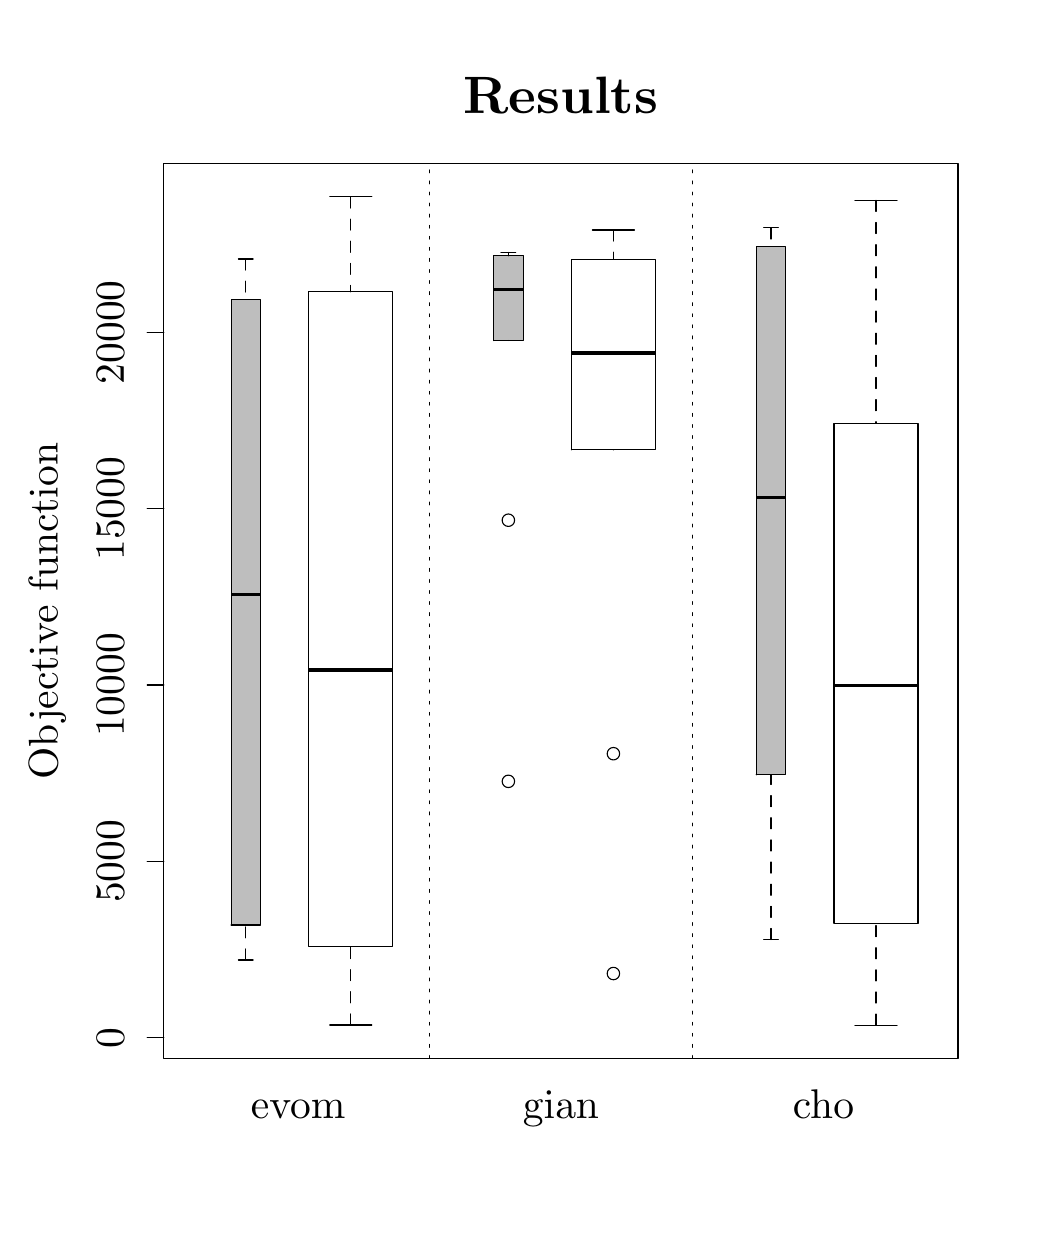
\begin{tikzpicture}[x=1pt,y=1pt]
\definecolor{fillColor}{RGB}{255,255,255}
\path[use as bounding box,fill=fillColor,fill opacity=0.00] (0,0) rectangle (361.35,433.62);
\begin{scope}
\path[clip] ( 49.20, 61.20) rectangle (336.15,384.42);
\definecolor{fillColor}{RGB}{190,190,190}

\path[fill=fillColor] ( 73.49,109.38) --
	( 84.12,109.38) --
	( 84.12,335.40) --
	( 73.49,335.40) --
	cycle;
\definecolor{drawColor}{RGB}{0,0,0}

\path[draw=drawColor,line width= 1.2pt,line join=round] ( 73.49,228.83) -- ( 84.12,228.83);

\path[draw=drawColor,line width= 0.4pt,dash pattern=on 4pt off 4pt ,line join=round,line cap=round] ( 78.81, 96.71) -- ( 78.81,109.38);

\path[draw=drawColor,line width= 0.4pt,dash pattern=on 4pt off 4pt ,line join=round,line cap=round] ( 78.81,350.04) -- ( 78.81,335.40);

\path[draw=drawColor,line width= 0.4pt,line join=round,line cap=round] ( 76.15, 96.71) -- ( 81.46, 96.71);

\path[draw=drawColor,line width= 0.4pt,line join=round,line cap=round] ( 76.15,350.04) -- ( 81.46,350.04);

\path[draw=drawColor,line width= 0.4pt,line join=round,line cap=round] ( 73.49,109.38) --
	( 84.12,109.38) --
	( 84.12,335.40) --
	( 73.49,335.40) --
	( 73.49,109.38);
\definecolor{fillColor}{RGB}{255,255,255}

\path[fill=fillColor] (101.58,101.70) --
	(131.94,101.70) --
	(131.94,338.19) --
	(101.58,338.19) --
	cycle;

\path[draw=drawColor,line width= 1.2pt,line join=round] (101.58,201.56) -- (131.94,201.56);

\path[draw=drawColor,line width= 0.4pt,dash pattern=on 4pt off 4pt ,line join=round,line cap=round] (116.76, 73.25) -- (116.76,101.70);

\path[draw=drawColor,line width= 0.4pt,dash pattern=on 4pt off 4pt ,line join=round,line cap=round] (116.76,372.45) -- (116.76,338.19);

\path[draw=drawColor,line width= 0.4pt,line join=round,line cap=round] (109.17, 73.25) -- (124.35, 73.25);

\path[draw=drawColor,line width= 0.4pt,line join=round,line cap=round] (109.17,372.45) -- (124.35,372.45);

\path[draw=drawColor,line width= 0.4pt,line join=round,line cap=round] (101.58,101.70) --
	(131.94,101.70) --
	(131.94,338.19) --
	(101.58,338.19) --
	(101.58,101.70);
\definecolor{fillColor}{RGB}{190,190,190}

\path[fill=fillColor] (168.38,320.56) --
	(179.01,320.56) --
	(179.01,351.13) --
	(168.38,351.13) --
	cycle;

\path[draw=drawColor,line width= 1.2pt,line join=round] (168.38,338.97) -- (179.01,338.97);

\path[draw=drawColor,line width= 0.4pt,dash pattern=on 4pt off 4pt ,line join=round,line cap=round] (173.70,320.56) -- (173.70,320.56);

\path[draw=drawColor,line width= 0.4pt,dash pattern=on 4pt off 4pt ,line join=round,line cap=round] (173.70,352.37) -- (173.70,351.13);

\path[draw=drawColor,line width= 0.4pt,line join=round,line cap=round] (171.04,320.56) -- (176.35,320.56);

\path[draw=drawColor,line width= 0.4pt,line join=round,line cap=round] (171.04,352.37) -- (176.35,352.37);

\path[draw=drawColor,line width= 0.4pt,line join=round,line cap=round] (168.38,320.56) --
	(179.01,320.56) --
	(179.01,351.13) --
	(168.38,351.13) --
	(168.38,320.56);

\path[draw=drawColor,line width= 0.4pt,line join=round,line cap=round] (173.70,255.64) circle (  2.25);

\path[draw=drawColor,line width= 0.4pt,line join=round,line cap=round] (173.70,161.28) circle (  2.25);
\definecolor{fillColor}{RGB}{255,255,255}

\path[fill=fillColor] (196.47,281.03) --
	(226.84,281.03) --
	(226.84,349.91) --
	(196.47,349.91) --
	cycle;

\path[draw=drawColor,line width= 1.2pt,line join=round] (196.47,316.10) -- (226.84,316.10);

\path[draw=drawColor,line width= 0.4pt,dash pattern=on 4pt off 4pt ,line join=round,line cap=round] (211.65,281.03) -- (211.65,281.03);

\path[draw=drawColor,line width= 0.4pt,dash pattern=on 4pt off 4pt ,line join=round,line cap=round] (211.65,360.49) -- (211.65,349.91);

\path[draw=drawColor,line width= 0.4pt,line join=round,line cap=round] (204.06,281.03) -- (219.24,281.03);

\path[draw=drawColor,line width= 0.4pt,line join=round,line cap=round] (204.06,360.49) -- (219.24,360.49);

\path[draw=drawColor,line width= 0.4pt,line join=round,line cap=round] (196.47,281.03) --
	(226.84,281.03) --
	(226.84,349.91) --
	(196.47,349.91) --
	(196.47,281.03);

\path[draw=drawColor,line width= 0.4pt,line join=round,line cap=round] (211.65, 91.83) circle (  2.25);

\path[draw=drawColor,line width= 0.4pt,line join=round,line cap=round] (211.65,171.27) circle (  2.25);
\definecolor{fillColor}{RGB}{190,190,190}

\path[fill=fillColor] (263.27,163.60) --
	(273.90,163.60) --
	(273.90,354.52) --
	(263.27,354.52) --
	cycle;

\path[draw=drawColor,line width= 1.2pt,line join=round] (263.27,263.84) -- (273.90,263.84);

\path[draw=drawColor,line width= 0.4pt,dash pattern=on 4pt off 4pt ,line join=round,line cap=round] (268.59,104.12) -- (268.59,163.60);

\path[draw=drawColor,line width= 0.4pt,dash pattern=on 4pt off 4pt ,line join=round,line cap=round] (268.59,361.25) -- (268.59,354.52);

\path[draw=drawColor,line width= 0.4pt,line join=round,line cap=round] (265.93,104.12) -- (271.24,104.12);

\path[draw=drawColor,line width= 0.4pt,line join=round,line cap=round] (265.93,361.25) -- (271.24,361.25);

\path[draw=drawColor,line width= 0.4pt,line join=round,line cap=round] (263.27,163.60) --
	(273.90,163.60) --
	(273.90,354.52) --
	(263.27,354.52) --
	(263.27,163.60);
\definecolor{fillColor}{RGB}{255,255,255}

\path[fill=fillColor] (291.36,110.06) --
	(321.73,110.06) --
	(321.73,290.69) --
	(291.36,290.69) --
	cycle;

\path[draw=drawColor,line width= 1.2pt,line join=round] (291.36,196.02) -- (321.73,196.02);

\path[draw=drawColor,line width= 0.4pt,dash pattern=on 4pt off 4pt ,line join=round,line cap=round] (306.54, 73.17) -- (306.54,110.06);

\path[draw=drawColor,line width= 0.4pt,dash pattern=on 4pt off 4pt ,line join=round,line cap=round] (306.54,371.21) -- (306.54,290.69);

\path[draw=drawColor,line width= 0.4pt,line join=round,line cap=round] (298.95, 73.17) -- (314.14, 73.17);

\path[draw=drawColor,line width= 0.4pt,line join=round,line cap=round] (298.95,371.21) -- (314.14,371.21);

\path[draw=drawColor,line width= 0.4pt,line join=round,line cap=round] (291.36,110.06) --
	(321.73,110.06) --
	(321.73,290.69) --
	(291.36,290.69) --
	(291.36,110.06);
\end{scope}
\begin{scope}
\path[clip] (  0.00,  0.00) rectangle (361.35,433.62);
\definecolor{drawColor}{RGB}{0,0,0}

\node[text=drawColor,rotate= 90.00,anchor=base,inner sep=0pt, outer sep=0pt, scale=  1.50] at ( 10.80,222.81) {Objective function};
\end{scope}
\begin{scope}
\path[clip] ( 49.20, 61.20) rectangle (336.15,384.42);
\definecolor{drawColor}{RGB}{0,0,0}

\path[draw=drawColor,line width= 0.4pt,dash pattern=on 1pt off 3pt ,line join=round,line cap=round] (145.23, 61.20) -- (145.23,384.42);

\path[draw=drawColor,line width= 0.4pt,dash pattern=on 1pt off 3pt ,line join=round,line cap=round] (240.12, 61.20) -- (240.12,384.42);
\end{scope}
\begin{scope}
\path[clip] (  0.00,  0.00) rectangle (361.35,433.62);
\definecolor{drawColor}{RGB}{0,0,0}

\node[text=drawColor,anchor=base,inner sep=0pt, outer sep=0pt, scale=  1.50] at ( 97.78, 39.60) {evom};

\node[text=drawColor,anchor=base,inner sep=0pt, outer sep=0pt, scale=  1.50] at (192.67, 39.60) {gian};

\node[text=drawColor,anchor=base,inner sep=0pt, outer sep=0pt, scale=  1.50] at (287.57, 39.60) {cho};
\end{scope}
\begin{scope}
\path[clip] (  0.00,  0.00) rectangle (361.35,433.62);
\definecolor{drawColor}{RGB}{0,0,0}

\node[text=drawColor,anchor=base,inner sep=0pt, outer sep=0pt, scale=  1.90] at (192.68,402.46) {\bfseries Results};
\end{scope}
\begin{scope}
\path[clip] (  0.00,  0.00) rectangle (361.35,433.62);
\definecolor{drawColor}{RGB}{0,0,0}

\path[draw=drawColor,line width= 0.4pt,line join=round,line cap=round] ( 49.20, 68.62) -- ( 49.20,323.53);

\path[draw=drawColor,line width= 0.4pt,line join=round,line cap=round] ( 49.20, 68.62) -- ( 43.20, 68.62);

\path[draw=drawColor,line width= 0.4pt,line join=round,line cap=round] ( 49.20,132.35) -- ( 43.20,132.35);

\path[draw=drawColor,line width= 0.4pt,line join=round,line cap=round] ( 49.20,196.08) -- ( 43.20,196.08);

\path[draw=drawColor,line width= 0.4pt,line join=round,line cap=round] ( 49.20,259.80) -- ( 43.20,259.80);

\path[draw=drawColor,line width= 0.4pt,line join=round,line cap=round] ( 49.20,323.53) -- ( 43.20,323.53);

\node[text=drawColor,rotate= 90.00,anchor=base,inner sep=0pt, outer sep=0pt, scale=  1.50] at ( 34.80, 68.62) {0};

\node[text=drawColor,rotate= 90.00,anchor=base,inner sep=0pt, outer sep=0pt, scale=  1.50] at ( 34.80,132.35) {5000};

\node[text=drawColor,rotate= 90.00,anchor=base,inner sep=0pt, outer sep=0pt, scale=  1.50] at ( 34.80,196.08) {10000};

\node[text=drawColor,rotate= 90.00,anchor=base,inner sep=0pt, outer sep=0pt, scale=  1.50] at ( 34.80,259.80) {15000};

\node[text=drawColor,rotate= 90.00,anchor=base,inner sep=0pt, outer sep=0pt, scale=  1.50] at ( 34.80,323.53) {20000};

\path[draw=drawColor,line width= 0.4pt,line join=round,line cap=round] ( 49.20, 61.20) --
	(336.15, 61.20) --
	(336.15,384.42) --
	( 49.20,384.42) --
	( 49.20, 61.20);
\end{scope}
\end{tikzpicture}

\caption{
Thick gray boxes represent the results of robot experiments;
Thick white boxes those of pseudo-reality; thin gray ones,
those of simulations.}
\label{fig:task1res}
\end{figure}

\begin{figure}[t]
\centering
% Created by tikzDevice version 0.12 on 2019-02-08 11:09:25
% !TEX encoding = UTF-8 Unicode
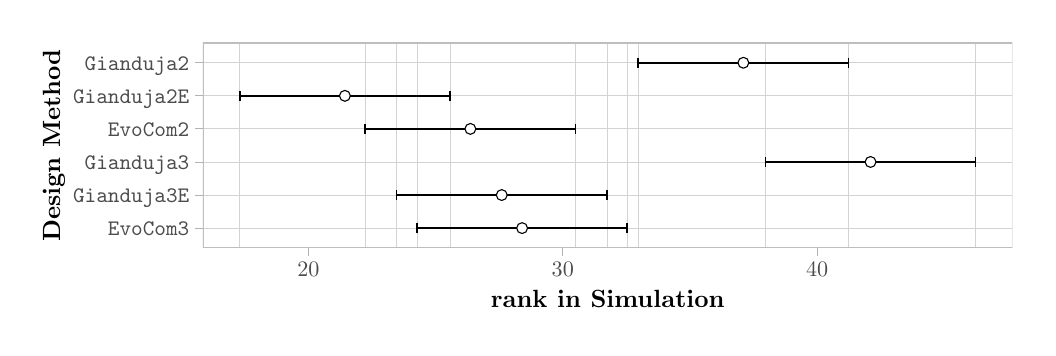
\begin{tikzpicture}[x=1pt,y=1pt]
\definecolor{fillColor}{RGB}{255,255,255}
\path[use as bounding box,fill=fillColor,fill opacity=0.00] (0,0) rectangle (361.35,108.41);
\begin{scope}
\path[clip] (  0.00,  0.00) rectangle (361.35,108.40);
\definecolor{drawColor}{RGB}{255,255,255}
\definecolor{fillColor}{RGB}{255,255,255}

\path[draw=drawColor,line width= 0.6pt,line join=round,line cap=round,fill=fillColor] (  0.00,  0.00) rectangle (361.35,108.40);
\end{scope}
\begin{scope}
\path[clip] ( 63.34, 28.81) rectangle (355.85,102.90);
\definecolor{fillColor}{RGB}{255,255,255}

\path[fill=fillColor] ( 63.34, 28.81) rectangle (355.85,102.90);
\definecolor{drawColor}{RGB}{211,211,211}

\path[draw=drawColor,line width= 0.3pt,line join=round] ( 63.34, 71.83) --
	(355.85, 71.83);

\path[draw=drawColor,line width= 0.3pt,line join=round] ( 63.34, 35.98) --
	(355.85, 35.98);

\path[draw=drawColor,line width= 0.3pt,line join=round] ( 63.34, 95.73) --
	(355.85, 95.73);

\path[draw=drawColor,line width= 0.3pt,line join=round] ( 63.34, 83.78) --
	(355.85, 83.78);

\path[draw=drawColor,line width= 0.3pt,line join=round] ( 63.34, 59.88) --
	(355.85, 59.88);

\path[draw=drawColor,line width= 0.3pt,line join=round] ( 63.34, 47.93) --
	(355.85, 47.93);

\path[draw=drawColor,line width= 0.2pt,line join=round] (197.95, 28.81) -- (197.95,102.90);

\path[draw=drawColor,line width= 0.2pt,line join=round] (296.60, 28.81) -- (296.60,102.90);

\path[draw=drawColor,line width= 0.2pt,line join=round] (152.61, 28.81) -- (152.61,102.90);

\path[draw=drawColor,line width= 0.2pt,line join=round] (216.64, 28.81) -- (216.64,102.90);

\path[draw=drawColor,line width= 0.2pt,line join=round] (342.55, 28.81) -- (342.55,102.90);

\path[draw=drawColor,line width= 0.2pt,line join=round] (209.29, 28.81) -- (209.29,102.90);

\path[draw=drawColor,line width= 0.2pt,line join=round] (121.98, 28.81) -- (121.98,102.90);

\path[draw=drawColor,line width= 0.2pt,line join=round] (220.63, 28.81) -- (220.63,102.90);

\path[draw=drawColor,line width= 0.2pt,line join=round] ( 76.64, 28.81) -- ( 76.64,102.90);

\path[draw=drawColor,line width= 0.2pt,line join=round] (140.67, 28.81) -- (140.67,102.90);

\path[draw=drawColor,line width= 0.2pt,line join=round] (266.58, 28.81) -- (266.58,102.90);

\path[draw=drawColor,line width= 0.2pt,line join=round] (133.32, 28.81) -- (133.32,102.90);
\definecolor{drawColor}{RGB}{0,0,0}

\path[draw=drawColor,line width= 0.6pt,line join=round] (197.95, 70.04) --
	(197.95, 73.62);

\path[draw=drawColor,line width= 0.6pt,line join=round] (197.95, 71.83) --
	(121.98, 71.83);

\path[draw=drawColor,line width= 0.6pt,line join=round] (121.98, 70.04) --
	(121.98, 73.62);

\path[draw=drawColor,line width= 0.6pt,line join=round] (296.60, 93.94) --
	(296.60, 97.53);

\path[draw=drawColor,line width= 0.6pt,line join=round] (296.60, 95.73) --
	(220.63, 95.73);

\path[draw=drawColor,line width= 0.6pt,line join=round] (220.63, 93.94) --
	(220.63, 97.53);

\path[draw=drawColor,line width= 0.6pt,line join=round] (152.61, 81.99) --
	(152.61, 85.58);

\path[draw=drawColor,line width= 0.6pt,line join=round] (152.61, 83.78) --
	( 76.64, 83.78);

\path[draw=drawColor,line width= 0.6pt,line join=round] ( 76.64, 81.99) --
	( 76.64, 85.58);

\path[draw=drawColor,line width= 0.6pt,line join=round] (216.64, 34.19) --
	(216.64, 37.77);

\path[draw=drawColor,line width= 0.6pt,line join=round] (216.64, 35.98) --
	(140.67, 35.98);

\path[draw=drawColor,line width= 0.6pt,line join=round] (140.67, 34.19) --
	(140.67, 37.77);

\path[draw=drawColor,line width= 0.6pt,line join=round] (342.55, 58.09) --
	(342.55, 61.67);

\path[draw=drawColor,line width= 0.6pt,line join=round] (342.55, 59.88) --
	(266.58, 59.88);

\path[draw=drawColor,line width= 0.6pt,line join=round] (266.58, 58.09) --
	(266.58, 61.67);

\path[draw=drawColor,line width= 0.6pt,line join=round] (209.29, 46.14) --
	(209.29, 49.72);

\path[draw=drawColor,line width= 0.6pt,line join=round] (209.29, 47.93) --
	(133.32, 47.93);

\path[draw=drawColor,line width= 0.6pt,line join=round] (133.32, 46.14) --
	(133.32, 49.72);

\path[draw=drawColor,line width= 0.4pt,line join=round,line cap=round,fill=fillColor] (159.97, 71.83) circle (  1.96);

\path[draw=drawColor,line width= 0.4pt,line join=round,line cap=round,fill=fillColor] (258.62, 95.73) circle (  1.96);

\path[draw=drawColor,line width= 0.4pt,line join=round,line cap=round,fill=fillColor] (114.63, 83.78) circle (  1.96);

\path[draw=drawColor,line width= 0.4pt,line join=round,line cap=round,fill=fillColor] (178.66, 35.98) circle (  1.96);

\path[draw=drawColor,line width= 0.4pt,line join=round,line cap=round,fill=fillColor] (304.57, 59.88) circle (  1.96);

\path[draw=drawColor,line width= 0.4pt,line join=round,line cap=round,fill=fillColor] (171.30, 47.93) circle (  1.96);
\definecolor{drawColor}{RGB}{190,190,190}

\path[draw=drawColor,line width= 0.6pt,line join=round,line cap=round] ( 63.34, 28.81) rectangle (355.85,102.90);
\end{scope}
\begin{scope}
\path[clip] (  0.00,  0.00) rectangle (361.35,108.41);
\definecolor{drawColor}{gray}{0.30}

\node[text=drawColor,anchor=base east,inner sep=0pt, outer sep=0pt, scale=  0.80] at ( 58.39, 69.08) {\texttt{EvoCom2}};

\node[text=drawColor,anchor=base east,inner sep=0pt, outer sep=0pt, scale=  0.80] at ( 58.39, 33.22) {\texttt{EvoCom3}};

\node[text=drawColor,anchor=base east,inner sep=0pt, outer sep=0pt, scale=  0.80] at ( 58.39, 92.98) {\texttt{Gianduja2}};

\node[text=drawColor,anchor=base east,inner sep=0pt, outer sep=0pt, scale=  0.80] at ( 58.39, 81.03) {\texttt{Gianduja2E}};

\node[text=drawColor,anchor=base east,inner sep=0pt, outer sep=0pt, scale=  0.80] at ( 58.39, 57.13) {\texttt{Gianduja3}};

\node[text=drawColor,anchor=base east,inner sep=0pt, outer sep=0pt, scale=  0.80] at ( 58.39, 45.18) {\texttt{Gianduja3E}};
\end{scope}
\begin{scope}
\path[clip] (  0.00,  0.00) rectangle (361.35,108.41);
\definecolor{drawColor}{gray}{0.70}

\path[draw=drawColor,line width= 0.3pt,line join=round] ( 60.59, 71.83) --
	( 63.34, 71.83);

\path[draw=drawColor,line width= 0.3pt,line join=round] ( 60.59, 35.98) --
	( 63.34, 35.98);

\path[draw=drawColor,line width= 0.3pt,line join=round] ( 60.59, 95.73) --
	( 63.34, 95.73);

\path[draw=drawColor,line width= 0.3pt,line join=round] ( 60.59, 83.78) --
	( 63.34, 83.78);

\path[draw=drawColor,line width= 0.3pt,line join=round] ( 60.59, 59.88) --
	( 63.34, 59.88);

\path[draw=drawColor,line width= 0.3pt,line join=round] ( 60.59, 47.93) --
	( 63.34, 47.93);
\end{scope}
\begin{scope}
\path[clip] (  0.00,  0.00) rectangle (361.35,108.41);
\definecolor{drawColor}{gray}{0.70}

\path[draw=drawColor,line width= 0.3pt,line join=round] (101.45, 26.06) --
	(101.45, 28.81);

\path[draw=drawColor,line width= 0.3pt,line join=round] (193.36, 26.06) --
	(193.36, 28.81);

\path[draw=drawColor,line width= 0.3pt,line join=round] (285.27, 26.06) --
	(285.27, 28.81);
\end{scope}
\begin{scope}
\path[clip] (  0.00,  0.00) rectangle (361.35,108.41);
\definecolor{drawColor}{gray}{0.30}

\node[text=drawColor,anchor=base,inner sep=0pt, outer sep=0pt, scale=  0.80] at (101.45, 18.35) {20};

\node[text=drawColor,anchor=base,inner sep=0pt, outer sep=0pt, scale=  0.80] at (193.36, 18.35) {30};

\node[text=drawColor,anchor=base,inner sep=0pt, outer sep=0pt, scale=  0.80] at (285.27, 18.35) {40};
\end{scope}
\begin{scope}
\path[clip] (  0.00,  0.00) rectangle (361.35,108.41);
\definecolor{drawColor}{RGB}{0,0,0}

\node[text=drawColor,anchor=base,inner sep=0pt, outer sep=0pt, scale=  0.90] at (209.60,  7.44) {\bfseries rank in Simulation};
\end{scope}
\begin{scope}
\path[clip] (  0.00,  0.00) rectangle (361.35,108.41);
\definecolor{drawColor}{RGB}{0,0,0}

\node[text=drawColor,rotate= 90.00,anchor=base,inner sep=0pt, outer sep=0pt, scale=  0.90] at ( 11.71, 65.86) {\bfseries Design Method};
\end{scope}
\end{tikzpicture}

\caption{Friedman test on the aggregated results of the three missions. The
  plot represents the average rank of the seven methods and their
  95\% confidence interval. }
\label{fig:friedmanSIM}
\end{figure}

\begin{figure}[t]
\centering
% Created by tikzDevice version 0.12 on 2019-01-19 16:45:08
% !TEX encoding = UTF-8 Unicode
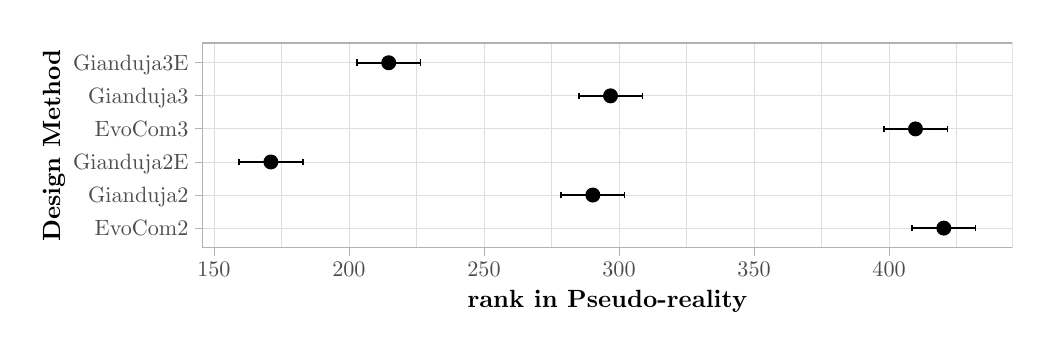
\begin{tikzpicture}[x=1pt,y=1pt]
\definecolor{fillColor}{RGB}{255,255,255}
\path[use as bounding box,fill=fillColor,fill opacity=0.00] (0,0) rectangle (361.35,108.41);
\begin{scope}
\path[clip] (  0.00,  0.00) rectangle (361.35,108.40);
\definecolor{drawColor}{RGB}{255,255,255}
\definecolor{fillColor}{RGB}{255,255,255}

\path[draw=drawColor,line width= 0.6pt,line join=round,line cap=round,fill=fillColor] (  0.00,  0.00) rectangle (361.35,108.40);
\end{scope}
\begin{scope}
\path[clip] ( 63.07, 28.81) rectangle (355.85,102.90);
\definecolor{fillColor}{RGB}{255,255,255}

\path[fill=fillColor] ( 63.07, 28.81) rectangle (355.85,102.90);
\definecolor{drawColor}{gray}{0.87}

\path[draw=drawColor,line width= 0.1pt,line join=round] ( 91.69, 28.81) --
	( 91.69,102.90);

\path[draw=drawColor,line width= 0.1pt,line join=round] (140.49, 28.81) --
	(140.49,102.90);

\path[draw=drawColor,line width= 0.1pt,line join=round] (189.28, 28.81) --
	(189.28,102.90);

\path[draw=drawColor,line width= 0.1pt,line join=round] (238.08, 28.81) --
	(238.08,102.90);

\path[draw=drawColor,line width= 0.1pt,line join=round] (286.87, 28.81) --
	(286.87,102.90);

\path[draw=drawColor,line width= 0.1pt,line join=round] (335.67, 28.81) --
	(335.67,102.90);

\path[draw=drawColor,line width= 0.3pt,line join=round] ( 63.07, 35.98) --
	(355.85, 35.98);

\path[draw=drawColor,line width= 0.3pt,line join=round] ( 63.07, 47.93) --
	(355.85, 47.93);

\path[draw=drawColor,line width= 0.3pt,line join=round] ( 63.07, 59.88) --
	(355.85, 59.88);

\path[draw=drawColor,line width= 0.3pt,line join=round] ( 63.07, 71.83) --
	(355.85, 71.83);

\path[draw=drawColor,line width= 0.3pt,line join=round] ( 63.07, 83.78) --
	(355.85, 83.78);

\path[draw=drawColor,line width= 0.3pt,line join=round] ( 63.07, 95.73) --
	(355.85, 95.73);

\path[draw=drawColor,line width= 0.3pt,line join=round] ( 67.30, 28.81) --
	( 67.30,102.90);

\path[draw=drawColor,line width= 0.3pt,line join=round] (116.09, 28.81) --
	(116.09,102.90);

\path[draw=drawColor,line width= 0.3pt,line join=round] (164.89, 28.81) --
	(164.89,102.90);

\path[draw=drawColor,line width= 0.3pt,line join=round] (213.68, 28.81) --
	(213.68,102.90);

\path[draw=drawColor,line width= 0.3pt,line join=round] (262.48, 28.81) --
	(262.48,102.90);

\path[draw=drawColor,line width= 0.3pt,line join=round] (311.27, 28.81) --
	(311.27,102.90);
\definecolor{drawColor}{RGB}{0,0,0}
\definecolor{fillColor}{RGB}{0,0,0}

\path[draw=drawColor,line width= 0.4pt,line join=round,line cap=round,fill=fillColor] (331.04, 35.98) circle (  2.50);

\path[draw=drawColor,line width= 0.4pt,line join=round,line cap=round,fill=fillColor] (204.22, 47.93) circle (  2.50);

\path[draw=drawColor,line width= 0.4pt,line join=round,line cap=round,fill=fillColor] ( 87.88, 59.88) circle (  2.50);

\path[draw=drawColor,line width= 0.4pt,line join=round,line cap=round,fill=fillColor] (320.81, 71.83) circle (  2.50);

\path[draw=drawColor,line width= 0.4pt,line join=round,line cap=round,fill=fillColor] (210.61, 83.78) circle (  2.50);

\path[draw=drawColor,line width= 0.4pt,line join=round,line cap=round,fill=fillColor] (130.45, 95.73) circle (  2.50);

\path[draw=drawColor,line width= 0.6pt,line join=round] (342.54, 34.78) --
	(342.54, 37.17);

\path[draw=drawColor,line width= 0.6pt,line join=round] (342.54, 35.98) --
	(319.54, 35.98);

\path[draw=drawColor,line width= 0.6pt,line join=round] (319.54, 34.78) --
	(319.54, 37.17);

\path[draw=drawColor,line width= 0.6pt,line join=round] (215.72, 46.74) --
	(215.72, 49.13);

\path[draw=drawColor,line width= 0.6pt,line join=round] (215.72, 47.93) --
	(192.72, 47.93);

\path[draw=drawColor,line width= 0.6pt,line join=round] (192.72, 46.74) --
	(192.72, 49.13);

\path[draw=drawColor,line width= 0.6pt,line join=round] ( 99.38, 58.69) --
	( 99.38, 61.08);

\path[draw=drawColor,line width= 0.6pt,line join=round] ( 99.38, 59.88) --
	( 76.38, 59.88);

\path[draw=drawColor,line width= 0.6pt,line join=round] ( 76.38, 58.69) --
	( 76.38, 61.08);

\path[draw=drawColor,line width= 0.6pt,line join=round] (332.32, 70.64) --
	(332.32, 73.03);

\path[draw=drawColor,line width= 0.6pt,line join=round] (332.32, 71.83) --
	(309.31, 71.83);

\path[draw=drawColor,line width= 0.6pt,line join=round] (309.31, 70.64) --
	(309.31, 73.03);

\path[draw=drawColor,line width= 0.6pt,line join=round] (222.11, 82.59) --
	(222.11, 84.98);

\path[draw=drawColor,line width= 0.6pt,line join=round] (222.11, 83.78) --
	(199.11, 83.78);

\path[draw=drawColor,line width= 0.6pt,line join=round] (199.11, 82.59) --
	(199.11, 84.98);

\path[draw=drawColor,line width= 0.6pt,line join=round] (141.95, 94.54) --
	(141.95, 96.93);

\path[draw=drawColor,line width= 0.6pt,line join=round] (141.95, 95.73) --
	(118.95, 95.73);

\path[draw=drawColor,line width= 0.6pt,line join=round] (118.95, 94.54) --
	(118.95, 96.93);
\definecolor{drawColor}{gray}{0.70}

\path[draw=drawColor,line width= 0.6pt,line join=round,line cap=round] ( 63.07, 28.81) rectangle (355.85,102.90);
\end{scope}
\begin{scope}
\path[clip] (  0.00,  0.00) rectangle (361.35,108.41);
\definecolor{drawColor}{gray}{0.30}

\node[text=drawColor,anchor=base east,inner sep=0pt, outer sep=0pt, scale=  0.80] at ( 58.12, 33.22) {EvoCom2};

\node[text=drawColor,anchor=base east,inner sep=0pt, outer sep=0pt, scale=  0.80] at ( 58.12, 45.18) {Gianduja2};

\node[text=drawColor,anchor=base east,inner sep=0pt, outer sep=0pt, scale=  0.80] at ( 58.12, 57.13) {Gianduja2E};

\node[text=drawColor,anchor=base east,inner sep=0pt, outer sep=0pt, scale=  0.80] at ( 58.12, 69.08) {EvoCom3};

\node[text=drawColor,anchor=base east,inner sep=0pt, outer sep=0pt, scale=  0.80] at ( 58.12, 81.03) {Gianduja3};

\node[text=drawColor,anchor=base east,inner sep=0pt, outer sep=0pt, scale=  0.80] at ( 58.12, 92.98) {Gianduja3E};
\end{scope}
\begin{scope}
\path[clip] (  0.00,  0.00) rectangle (361.35,108.41);
\definecolor{drawColor}{gray}{0.70}

\path[draw=drawColor,line width= 0.3pt,line join=round] ( 60.32, 35.98) --
	( 63.07, 35.98);

\path[draw=drawColor,line width= 0.3pt,line join=round] ( 60.32, 47.93) --
	( 63.07, 47.93);

\path[draw=drawColor,line width= 0.3pt,line join=round] ( 60.32, 59.88) --
	( 63.07, 59.88);

\path[draw=drawColor,line width= 0.3pt,line join=round] ( 60.32, 71.83) --
	( 63.07, 71.83);

\path[draw=drawColor,line width= 0.3pt,line join=round] ( 60.32, 83.78) --
	( 63.07, 83.78);

\path[draw=drawColor,line width= 0.3pt,line join=round] ( 60.32, 95.73) --
	( 63.07, 95.73);
\end{scope}
\begin{scope}
\path[clip] (  0.00,  0.00) rectangle (361.35,108.41);
\definecolor{drawColor}{gray}{0.70}

\path[draw=drawColor,line width= 0.3pt,line join=round] ( 67.30, 26.06) --
	( 67.30, 28.81);

\path[draw=drawColor,line width= 0.3pt,line join=round] (116.09, 26.06) --
	(116.09, 28.81);

\path[draw=drawColor,line width= 0.3pt,line join=round] (164.89, 26.06) --
	(164.89, 28.81);

\path[draw=drawColor,line width= 0.3pt,line join=round] (213.68, 26.06) --
	(213.68, 28.81);

\path[draw=drawColor,line width= 0.3pt,line join=round] (262.48, 26.06) --
	(262.48, 28.81);

\path[draw=drawColor,line width= 0.3pt,line join=round] (311.27, 26.06) --
	(311.27, 28.81);
\end{scope}
\begin{scope}
\path[clip] (  0.00,  0.00) rectangle (361.35,108.41);
\definecolor{drawColor}{gray}{0.30}

\node[text=drawColor,anchor=base,inner sep=0pt, outer sep=0pt, scale=  0.80] at ( 67.30, 18.35) {150};

\node[text=drawColor,anchor=base,inner sep=0pt, outer sep=0pt, scale=  0.80] at (116.09, 18.35) {200};

\node[text=drawColor,anchor=base,inner sep=0pt, outer sep=0pt, scale=  0.80] at (164.89, 18.35) {250};

\node[text=drawColor,anchor=base,inner sep=0pt, outer sep=0pt, scale=  0.80] at (213.68, 18.35) {300};

\node[text=drawColor,anchor=base,inner sep=0pt, outer sep=0pt, scale=  0.80] at (262.48, 18.35) {350};

\node[text=drawColor,anchor=base,inner sep=0pt, outer sep=0pt, scale=  0.80] at (311.27, 18.35) {400};
\end{scope}
\begin{scope}
\path[clip] (  0.00,  0.00) rectangle (361.35,108.41);
\definecolor{drawColor}{RGB}{0,0,0}

\node[text=drawColor,anchor=base,inner sep=0pt, outer sep=0pt, scale=  0.90] at (209.46,  7.44) {\bfseries rank in Pseudo-reality};
\end{scope}
\begin{scope}
\path[clip] (  0.00,  0.00) rectangle (361.35,108.41);
\definecolor{drawColor}{RGB}{0,0,0}

\node[text=drawColor,rotate= 90.00,anchor=base,inner sep=0pt, outer sep=0pt, scale=  0.90] at ( 11.71, 65.86) {\bfseries Design Method};
\end{scope}
\end{tikzpicture}

\caption{Friedman test on the aggregated results of the three missions. The
  plot represents the average rank of the seven methods and their
  95\% confidence interval. }
\label{fig:friedmanPR}
\end{figure}


\end{document}
